\chapter{Funções}\label{cap:Funcoes}

\epigraph{``Nada que vale a pena é fácil''.}{Eric Cartman,  South Park}

\epigraph{``O ego é o pior inimigo do Eu, mas o Eu é o melhor amigo do ego... O ego é um péssimo senhor, mas é um ótimo servidor''.}{Bhagavad Gita}

\section{Conceitos, Definições e Nomenclaturas}\label{sec:FuncoesConceitoDefinicaoNomenclaturas}

Após o conceito importantíssimo de conjunto o componente mais importante na matemática é provavelmente a noção de função, o autor deste manuscrito não hesita em afirmar que você leitor com certeza já teve contato com a ideia de função, seja em seus curso do primário, secundário ou mesmo mais recentemente em suas disciplinas de nível superior tais como cálculo diferencial e integral ou alguma disciplina de física. 

Dado este encontra anterior do leitor sobre o assunto o autor fica confortável a pedir que leitor faça uma pequena pausa e tente lembrar de seus cursos anteriores e respondo para si mesmo ao questionamento: \textbf{o que é uma função}?

Bem, para muitos físicos, estatísticos e alguns matemáticos (não todos\footnote{Um visão interessante é aquela apontada em \cite{levin2021}, que descreve uma função como sendo um objeto com quatro descrições simultâneas: uma algébrica, uma numérica, uma gráfica e uma descritiva (ou em palavras).}), uma função é vista meramente como sendo um mapeamento (ou transformação) entre os elementos de dois conjuntos \cite{abe1991-TC}. Por outro lado, em obras tais como \cite{sussana2010-MD, lipschutz1971-Topo, lipschutz1978-TC, lipschutz2013-MD, Gerard2021discreta} uma função é vista como uma caso particular de relação entre dois conjuntos, ou seja, em última análise para esse grupo de pessoas uma função é exatamente um conjunto\footnote{Para melhor entender essa visão talvez o leitor deva revistar os Capítulos \ref{cap:Conjuntos} e \ref{cap:Relacoes} e revisar as definições apresentadas nos mesmo.}. Já em \cite{edward2019-MD, fmcbook} é apresentado uma visão mais mecanicista da ideia de função, essa visão captura a ideia de função enquanto uma máquina\footnote{Para cientistas da computação os termos máquina e programa são sinônimos.} (ou caixa preta) que transforma as entradas (\textit{inputs}) em saídas (\textit{outputs}), essa visão é ilustrada pela Figura \ref{fig:FuncaoBlackBox}. 

Há também a ideia de função como sendo uma estrutura \cite{judith2021}, com componentes bem estabelecidos. Essa visão é capaz (como será mostrado a seguir) de captura todas as outras ideias de função.  Neste manuscrito a formalização da ideia de função como sendo uma estrutura será apresentada de forma gradual trançando paralelos com as linguagens de programação que possuam um sistema de tipos, isso será adotado para tornar o texto mais didático e interessante ao leitor de computação, além disso, irá aproximar os tópicos teóricos (as funções) dos tópicos práticos (programação) cujo leitor desse manuscrito naturalmente tem contato e provável interesse. Entretanto, esse forma de apresentação não será menos rigorosa que outras fontes bibliográficas, na verdade será o oposto, o texto aqui apresentado tende a ser mais preciso e detalhado que a apresentação rasa feita em \cite{judith2021}, por exemplo.

\begin{figure}[h]
	\centering
	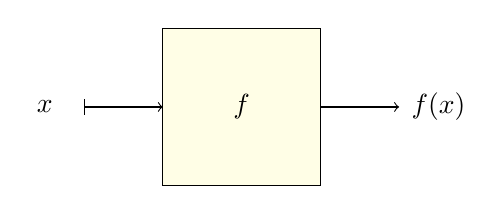
\begin{tikzpicture}
		\draw [rounded corners=0mm, fill=yellow!10]  (-1,1)--(-1,-1)--(1,-1)--(1,1)--cycle;
		\draw[->]  (1.0,0) -- (2.0,0.0);
	    \draw[|->]  (-2.0,0) -- (-1.0,0.0);
		\node (f) at (0,0) {$f$};
		\node (fx) at (2.5,0) {$f(x)$};
		\node (x) at (-2.5,0) {$x$};
	\end{tikzpicture}
	\caption{Visão de uma função de uma variável enquanto uma máquina (ou caixa preta).}
	\label{fig:FuncaoBlackBox}
\end{figure}

Este manuscrito irá iniciar o estudo sobre funções  apresentado ao leitor a ideia básica de assinatura de função, isto é, a seguir será apresentado a estrutura sintática que descreve as funções, ou seja, o componente descritivo mencionado em \cite{levin2021}.

\begin{definition}[Assinatura de Função]\label{def:AssinaturaFuncao}
	Sejam $A$ e $B$ conjuntos a assinatura da função de $A$ em $B$ nomeada como $f$ corresponde a uma palavra da forma $f: A \rightarrow B$.
\end{definition}

Note que a Definição \ref{def:AssinaturaFuncao} permite facilmente deduzir que em qualquer função existem três componentes básicos, sendo eles: um nome (rótulo ou símbolo funcional), um conjunto de partida e um conjunto de chegada. Por convenção, o nome de uma função deve ser sempre iniciado por caracteres latinos, no caso de usar índices apenas o último caractere do nome deve ser indexado.

\begin{example}\label{exe:AssinaturaFuncao}
	São exemplos de assinaturas de funções:
	\begin{itemize}
		\item[(a)] $g : \mathbb{N} \rightarrow \mathbb{Z}$.
		\item[(b)] $sqrt : \mathbb{R} \rightarrow \mathbb{R}$.
		\item[(c)] $k_1 : A \times B \rightarrow \mathbb{C}$.
		\item[(d)] $loc_2 : D \rightarrow \mathbb{R} \times \{0,1\}$.
		\item[(e)] $min : \mathbb{R}^n \rightarrow \mathbb{R}$.
		\item[(f)] $BUSCA : \mathbb{Z}^n \times \mathbb{Z} \rightarrow \{0,1\}$.
		\item[(g)] $BUSCA : \mathbb{R}^n \times \mathbb{R} \rightarrow \{0,1\}$.
	\end{itemize}
\end{example}

Diversas linguagens de programação tais como C, C++ e Java apresentam a possibilidade de definir assinaturas de funções, na linguagem C por exemplo as assinaturas de funções que compõem uma biblioteca são reunidas em um arquivo de \textit{header}, isto é, um arquivo com a extensão .h, para mais detalhes consulte \cite{paulo2009algoritmos}.  

\begin{figure}[h]
	\begin{lstlisting}[style=mystyle]
		// Assinaturas
		int reverse(int x);
		unsigned int strlen (char *x);
		int strcmp (char *x, char *y);
		char *strcpy (char *y, char *x);
	\end{lstlisting}
	\caption{Exemplo de um Arquivo .h da linguagem C.}
\end{figure}


Um conceito indiretamente esboçado pela ideia de assinatura de função, é o de tipagem da função 

\begin{remark}
	O leitor deve observar que apesar das assinaturas nos itens (f) e (g) do Exemplo \ref{exe:AssinaturaFuncao} terem o mesmo nome, elas não são iguais, pois diferem no conjunto de partida, e assim não são a mesma assinatura. Esse tipo de cenário na computação recebe o nome de sobrecarga, isto é, o símbolo funcional $BUSCA$ está sobrecarregado para identificar duas funções distintas.
\end{remark}

Como dito anteriormente una função pode ser vista como uma máquina que transforma entradas em saídas, mas note que para que isso aconteça a máquina deve de alguma forma realizar ações sobre a entrada, ou seja, a máquina deve ``operar'' sobre a entrada. Esse conceito de como a máquina deve operar sobre as entradas é descrito por uma propriedade $P$ que define uma relação de construção\footnote{Alguns texto usam a nomenclatura lei de formação, ver por exemplo \cite{carmo2013}.}

\begin{definition}[Relação de construção]\label{def:RelacaoConstrucao}
	Dado dois conjuntos $A$ e $B$ e seja $x \in A$ e $y \in B$ a relação de construção definida por uma propriedade $P$ corresponde  ao seguinte conjunto 
	$$\varepsilon = \{(x, y)\mid P\}$$ tal que $\varepsilon$ satisfaz a seguinte condição: se $(x, y_1), (x, y_2) \in \varepsilon$, então $y_1 = y_2$.
\end{definition}

Note que a Definição \ref{def:RelacaoConstrucao} apenas descreve que as entradas (as variáveis) $x_1, \cdots, x_n$ se relacionam como uma única saída $y$ por uma certa propriedade $P$.

\begin{example}\label{exe:RelacaoConstrucao}
	São exemplos de relações de construção:
	\begin{itemize}
		\item[(a)] $\{(x, y) \in \mathbb{R}^2 \mid y = \log_2(x + 1)\}\}$
		\item[(b)] $\{(w_1w_2w_3\cdots w_m, y) \in E^2 \mid y = w_3\cdots w_mw_1w_2\}$ onde $E$ é o conjunto de todas as palavras do português com três letras ou mais e $w_i$ representa o $i$-ésimo símbolo de uma palavra $w$.
		\item[(c)] $\{(x, y) \in \mathbb{N}^2 \mid y = 14\}$.
		\item[(d)] $\Big\{(x_1, x_2, x_3, y) \in \mathbb{R} \times \mathbb{R} \times \mathbb{R}^*_+ \times \mathbb{R} \mid y = \sqrt[x_3]{\displaystyle\frac{1}{2}x_1 + x_2}\Big\}$.
	\end{itemize}
	Não são exemplos de relações de construção:
	\begin{itemize}
		\item[(e)] $\{(x, y) \in N_P \times I_P\}$ onde $N_P$ é o conjunto de todos os nomes de pessoas e $I_P$ é o conjunto de naturais que representam idades, note que em tal relação é permitido que $(\text{Fátima}, 10), (\text{Fátima}, 55)$ estejam nesse conjunto, portanto, esse conjunto não satisfaz a Definição \ref{def:RelacaoConstrucao}.
		\item[(f)] $\{(x, y) \in \mathbb{R} \sqrt{y} = x\}$, note que $(5, 25)$ e $(-5, 25)$ pertence a tal conjunto e, portanto, esse conjunto não satisfaz a Definição \ref{def:RelacaoConstrucao}.
	\end{itemize}
\end{example}

\begin{remark}
	O item (c) do Exemplo \ref{exe:RelacaoConstrucao} é um caso interessante, a propriedade da relação descreve que para qualquer entrada $x$ a mesma sempre irá devolver como resposta um $y = 14$, ou seja, para todo $x$ tem-se que o par $(x, 14)$ está na relação. Esse tipo de relação de construção será aqui chamada de \textbf{relação de construção constante}.    
\end{remark}

Agora que foram apresentados estes conceitos fundamentais pode-se continuar o desenvolvimento deste texto com a formalização da ideia de função.

\begin{definition}[Função]
	Dado uma assinatura $f: A \rightarrow B$ e seja $\varepsilon \subseteq A \times B$ uma relação de construção, a estrutura $\langle f: A \rightarrow B, \varepsilon \rangle$ é uma função.
\end{definition}

% Susam, lipstick (topo),  ver como relação